\subsection{Launch}
% Spiegare come facciamo spawnare i 2 agenti: entrambi dal main con flag isMaster = true / false
The multi-agent system is handled by launching the two agents in the \texttt{mainMulti.js} file simultaneously. The agent have different \texttt{DeliverooClient} and \texttt{Me} objects but the same objects for all the memory (\texttt{ParcelStore}, \texttt{MapStore}, \dots).

\subsubsection*{Launch Command}
Once you have configured the \texttt{.env} file, start the script by running:
\begin{verbatim}
npm run start-multi
\end{verbatim}




\subsection{Coordination}
\subsubsection*{Shared memory}
% Spiegare la memoria condivisa come funziona (gli passiamo la stessa zona di memoria)
By passing the same memory location to all the agents, the whole memory is shared between them and they can write and read in the same location, without the need to exchange messages.

\subsubsection*{Map division}
% Spiegare k-means per dividere la mappa
The map is divided equally between the agents, so they cover only their part and increase their efficiency. The division affects only the spawn tiles, so when performing an \textit{Explore} action, the agent only goes to one of the tiles that are assigned to it. \\

\noindent To split the map, the k-means algorithm is used: it is an unsupervised clustering algorithm that tries to make $k$ clusters (in this case 2) of tiles to assign one of them to each agent. If the algorithm cannot find a good split, it tries again a few times. If no solution is found, each agent can navigate the entire map for its explorations. 

\subsubsection*{Pickup parcels}
% Spiegare come si gestiscono gli agenti per decidere chi va a prendere la parcel
Each agent, in the \texttt{generateDesire} step, calculates the score for itself and for its own teammate. A desire is added to the list of possible intentions if its own score is higher than its teammate's, then the \texttt{filterIntentions} step is performed as usual. In this way, no parcel is contended by both agents simultaneously, reducing redundant actions and avoiding collisions due to conflicting goals.


\subsubsection*{Parcels exchange}
% Spiegare come facciamo lo scambio di parcels (tipo quando c'è il corridoio largo 1)
Sometimes it is necessary that agents collaborate to drop off parcels in a base that is reachable by only one of the agents: for instance, if there is a corridor of width equal to 1 tile and the agents can only move in one direction, up or down.

If an agent is carrying some parcels and detects its teammate in a neighbor tile of its current location, the agent which is further from the base drops the parcels and goes away from that location, freeing the tile. It communicates his drop action to the other agent within the shared memory; the other agent can now consider picking up those parcels, always calculating the potential score of its action.

A simple representation of this sequence of actions can be visualized in the figure \ref{fig:exchange}.

% Immagine per spiegare il parcel exchange
\begin{figure}
    \centering
    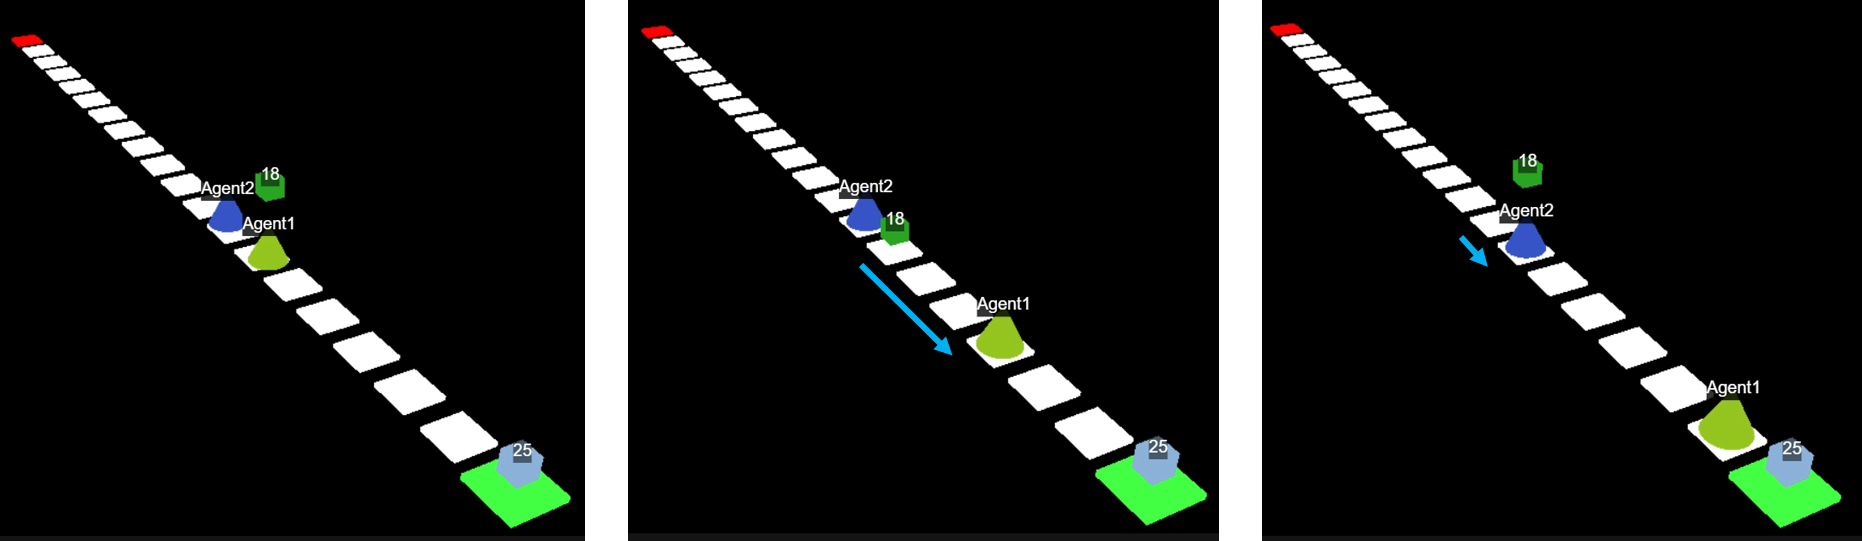
\includegraphics[width=\linewidth]{Images/exchange.png}
    \caption{Parcel exchange}
    \captionsetup{font=footnotesize}
    \caption*{The \textit{Agent1} detects its teammate, drops the parcels and goes away. The \textit{Agent2} goes to pickup the dropped parcels and will then deliver them to the base}
    \label{fig:exchange}
\end{figure}

% Spiegare se rimane bloccato
Sometimes an agent gets stuck because it cannot move in any direction, because it is blocked by his teammate. If this happens, it tells the other agent to move (through shared memory); the other agent pushes an intention with highest priority and moves away a few tiles, so the first agent has space to move and exchange the parcels correctly.


\subsection{Results in the Challenge 2}



Althought we placed 8\textsuperscript{th} among 14 teams, we further refined our code introducing the following new features:

\begin{itemize}
  \item \textbf{Map Partitioning via k‐Means:}  
    On the first game loop, we now optionally split the map between agents using k‐means (configurable with \texttt{USE\_MAP\_DIVISION}, \texttt{MAX\_TRIES\_KMEANS}, etc.). This ensures that each agent is responsible for its own sector, reducing overlap and improving parcel coverage.

  \item \textbf{Dynamic Base Reallocation and Path Fallback:}  
    We added a resilient \texttt{getBasePath(target)} routine that:  
    \begin{itemize}
      \item Attempts to compute a path to the given base tile.
      \item After a configurable number of failed tries (\texttt{BASE\_TRIES}), temporarily removes the blocked base tile from the map, waits \texttt{BASE\_REMOVAL\_TIME}, then restores it.
      \item Recomputes the nearest available base via \texttt{mapStore.nearestBase(this.me)} and updates \texttt{currentNearestBase}.
      \item Retries pathfinding up to \texttt{BASE\_SWITCH\_MAX\_TRIES} before giving up.
    \end{itemize}
\end{itemize}


